\documentclass[a4paper,14pt,russian]{extreport} \usepackage{extsizes}
\usepackage{cmap} 
\usepackage[T2A]{fontenc}
\usepackage[utf8]{inputenc}
\usepackage[russian]{babel}
\usepackage{pscyr}
\usepackage[warn]{mathtext} 
\usepackage{amsmath, amsfonts}
\usepackage{graphicx}

\begin{document}
	\chapter{Синтез управления}
	\section{Идентификация}
	\subsection{Системы координат}
	Всего у нас будет 3 системы координат: 
	\begin{enumerate}
		\item Связанная с основанием робота - базовая система координат. Центр системы координат выберем следующим образом: он будет находиться на пересечении оси вращения первого джоинта и горизональной плоскости, проходящей через ось вращения второго. Такое начало координат заложенно производителем. 
		\item Связанная с центром фланца рабочего инструмента.
		\item Связанная с силомоментным датчиком. 		
	\end{enumerate}
	Датчик закреплён на фланце робота таким образом, что оси z у них совпадают, систему координат, связанную с датчиком можно получить, повернув систему координат, связанную с фланцем, на угол $\frac{\pi}{2}$.
	В итоге для реализации управления нам необходимо составить матрицы прехода из первой системы координат во вторую и из второй - в третью.
	Обозначим матрицу перехода из первой системы во вторую ${M_{p12}}$, из второй в третью - ${M_{p23}}$.	
	\subsection{Нахождение матрицы перехода 1-2}
	Для нахождения матрицы перехода из первой системы во вторую можно воспользоваться одним из двух способов: 
	\begin{enumerate}
		\item Углы Эйлера в $zyz$ конвенции
		\item Прямая задача кинематики
	\end{enumerate}
	\paragraph{Углы Эйлера}
	От контроллера Kawasaki мы можем в режиме реального времени мы получаем координаты $X,Y,Z$ и углы Эйлера $O, A, T$ в $zyz$ конвенции (Рисунок 1.1). По этим координатам мы можем построить матрицу перехода из первой системы координат во вторую:
	
	${M_{p12}}=\begin{bmatrix} 
	cOcAcT-sOsT & -cOcAcT-sOcT & cOsA & X \\ 
	sOcAcT+cOsT & -sOcAsT+cOcT & sOsA & Y\\
	-sAsT & sAsT & cA & Z \\
	0 & 0 & 0 & 1
	\end{bmatrix}$ 
	
	\begin{figure}[h!]
		\centering		 
		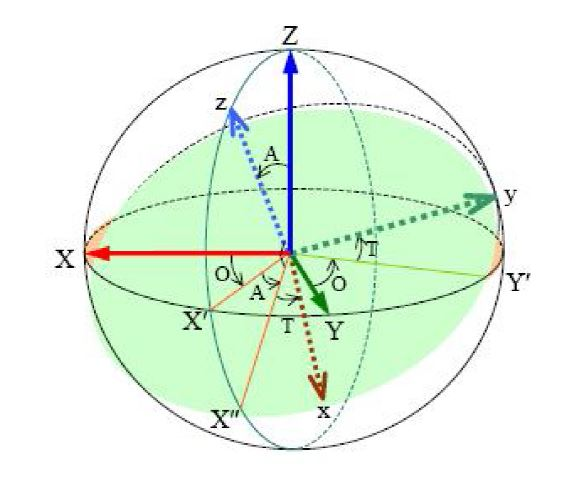
\includegraphics[width=6in]{./img/img21.JPG}	
		\caption{
		\textbf{$ZYZ$ конвенция углов Эйлера
			}     
		}
		\label{fig_img13}
	\end{figure}	
	\paragraph{Прямая задача кинематики}
	Методом Денавита-Хартенберга определим кинематические параметры каждого звена манипулятора. Значения параметров представлены в Таблице 1.1, кинематическая схема на рисунке 1.2. 
	
	Обобщённую координату $i$-го джоинта обозначим как $\theta_{i}$.
	Т.к. ось вращения первого джоинта направлена вертикально вниз, а z в базовой системе координат направлена вертикально вверх, было введено дополнительное преобразование из базовой системы координат в систему отсчёта первого джоинта.
	
	\begin{figure}[h!]
		\centering		 
		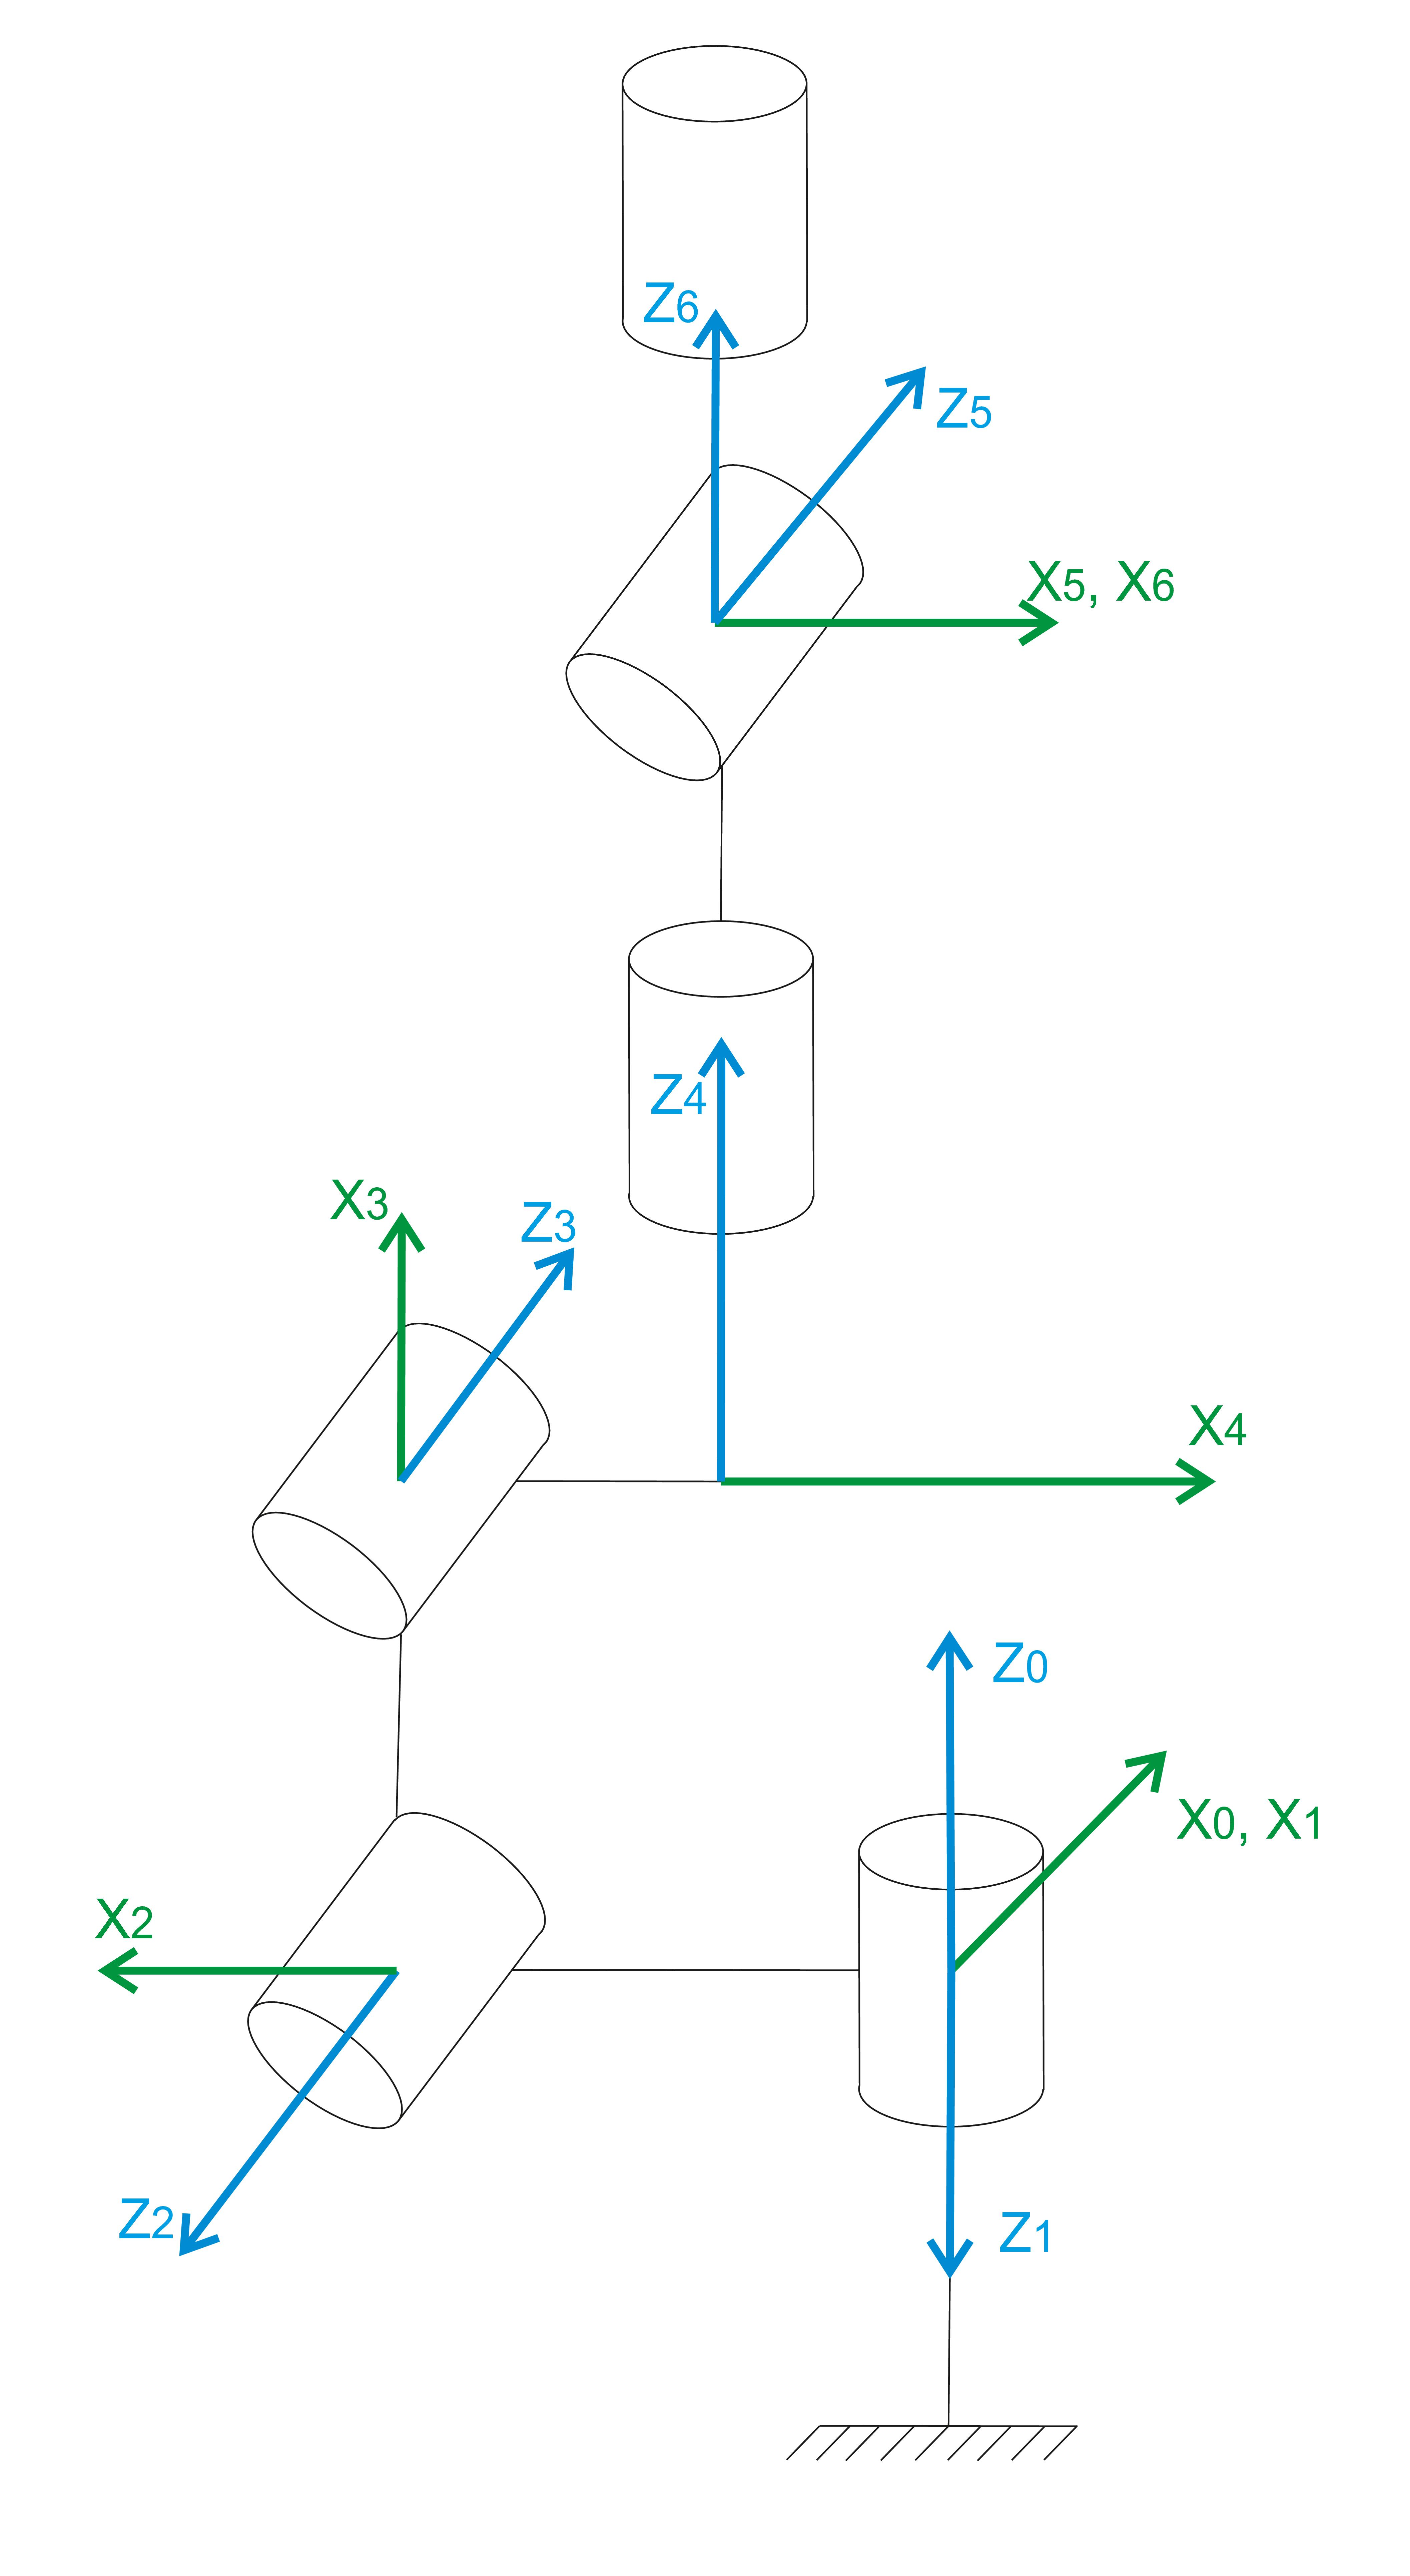
\includegraphics[width=3in]{./img/img31.JPG}	
		\caption{
			\textbf{Кинематическая схема
			}     
		}
		\label{fig_img14}
	\end{figure}
	
	 \begin{table}[h!]
	 	\caption{Кинематические звенья} 
	 	\label{tab_kaw_klass}
	 	\centering
	 	\begin{tabular}{|c|c|c|c|c|}	
	 		
	 		\hline № Звена & $\theta_{i}$  & $d_{i}$ & 	$a_{i}$ & $\alpha_{i} $\\
	 		\hline	0 &  0                  & 0    & 0     & $pi$ \\
	 		\hline	1 &  $\theta_{1}-pi/2$  & 0    & 0.1   & $pi/2$ \\
	 		\hline	2 &  $\theta_{2}-pi/2$  & 0    & 0.45  & $pi $ \\
	 		\hline	3 &  $\theta_{3}+pi/2$  & 0    & 0.04  & $pi/2$  \\
	 		\hline	4 &  $\theta_{4}$       & 0.45 & 0     & $-pi/2 $  \\
	 		\hline	5 &  $\theta_{5}$       & 0    & 0     &$ pi/2$ \\ 
	 		\hline	6 &  $\theta_{6} +pi/2$ & 0.1  & 0      & 0  \\		
	 		\hline
	 	\end{tabular} 
	 \end{table}
	
	Для $i$-го кинематического звена матрица перехода имеет вид: 
	\newline
	\centering
 	$A_{i} =\begin{bmatrix}
 	c \theta & -s \theta c \alpha & s \theta s\alpha&   c \theta a\\
 	s\theta & c\theta c\alpha & -c\theta s\alpha & s \theta a\\
 	0       &    s\alpha   &         c\alpha &             d\\
 	0       &    0          &           0    &                  1\\
	 \end{bmatrix}$ 
	\flushleft
	Тогда ${M_{p12}}=A_{0}A_{1}A_{2}A_{3}A_{4}A_{5}A_{6}$
	\subsection{Нахождение матрицы перехода 2-3}
	Т.к. матрица перехода 2-3 постоянна и имеет тривиальную форму, объявим её как константу:
	${M_{p12}}=\begin{bmatrix}
		 0 &-1&0&0\\ 1&0&0&0\\0 &0&1&0\\0&0&0&1\\
	\end{bmatrix}$
	\section{Обработка Сил}
	\subsection{Компенсация внутренних силовых напряжений}
	Т.к. монтаж датчика на фланец осуществлён совместно со схватом за счёт жёсткой фиксации, то возникают внутреннее давление которое порождает паразитные показания силы. 
	Для определения паразитных сил зафиксируем фланец робота в двух положениях: вертикально вверх и вертикально вниз. Получены следующие значения: 
	
	$\begin{pmatrix}
		-12.5 \\ 0 \\ -50\\
	\end{pmatrix}$ - для ориентации вертикально вверх
	
	$\begin{pmatrix}
	-12.5 \\ 0 \\ 10\\
	\end{pmatrix} $- для ориентации  вертикально вниз.
	
	Отсюда получаем, что внутреннее напряжение равно по оси $x$ 12.5H, а по оси $z$ -20H. Учитывая, что инструмент и монтажные элементы весят примерно 3кг, делаем вывод о правильных расчётах.
	
	В результате получаем вектор внутренних напряжений: 
	$F_{v}=\begin{pmatrix}
	-12.5 \\ 0 \\ -20\\
	\end{pmatrix} $
	\subsection{Компенсация силы тяжести}
	Обозначим матрицу перехода из системы координат датчика в базовую систему координат как ${M_{p13}}={M_{p12}}{M_{p23}}$.
	Т.к. сила тяжести направлена всегда вертикально вниз, то мы знаем вектор силы тяжести в базовой системе координат. Т.о. нам необходимо перевести вектор силы тяжести из базовой системы координат в систему координат датчика. 
	$F_{1} = \begin{pmatrix}
				0 \\ 0 \\ -30\\
			 \end{pmatrix}$, тогда в системе координат датчика $F_{g}=M_{13}^{-1} F_{1}$.
	\subsection{Перевод измерений датчика в базовую систему координат}
	Пусть $F_{0}$ - вектор сил, полученный с датчика. Тогда вектор показаний $F_{r}$, в котором уже скомпенсированны внутренние напряжения и сила тяжести:
	$F_{r}=	F_{0}-F_{v}-F_{g}$.
	
	Тогда показания датчика в базовой системе координат будут следующими:
	$F_{r}^*=M_{13}F_{r}$
	\section{Обработка Моментов}
	\subsection{Компенсация внутренних напряжений}
	По причинам, описанным в п1.2.1 в системе при ориентации вертикально вверх (все моменты, порождённые внешними силами, должны быть равны 0)
	мы получаем ненулевые значения. 
	Обозначим вектор внутренних моментов как $M_{v}$, тогда 
	$M_{v}= \begin{pmatrix}
				-0.34 \\ -0.18 \\ 0.52\\
			\end{pmatrix}$
	\subsection{Компенсация момента силы тяжести}
	Для того, чтобы скомпенсировать момент силы тяжести, введём вектор, соединяющий центр фланца и центр тяжести инструмента при ориентированном вертикально вверх инструменте:
	
	$r_{c_0} =  \begin{pmatrix}
			  0 \\ 0 \\ 0.07\\
			  \end{pmatrix}$

	тогда вектор соединяющий центр фланца и центр тяжести в произвольной конфигурации робота $r_{c}$ будет равен $M_{13}r_{c_0}$.
	
	Тогда момент силы тяжести в произвольном конфигурации в базовой системе координат равен в базовой системе координат $M_{g_0}=r{c}\times\begin{pmatrix}
	0 \\ 0 \\ -30\\
	\end{pmatrix}$
	
	В системе координат датчика тогда момент будет:
	
	$M_{g}=M_{13}^{-1}M_{g_0}$
	
	\subsection{Перевод измерений датчика в систему обобщённых координат}
	Пусть $M_{0}$ - вектор моментов, полученный с датчика. Тогда вектор показаний $M_{r}$, в котором уже скомпенсированны внутренние напряжения и сила тяжести:
	$M_{r}=	M_{0}-M_{v}-M_{g}$.		
	
	Наше управление будет построено следующим образом: возьмём первые четыре джоинта, будем последовательно переходить от системы координат шестого джоинта к системе координат третьего джоинта.
	
	 Перед каждым переходом $z$ координату вектора моментов будем сохранять в качестве приведённого момента $m_{i}$. После чего следует обнулить $z$ - координату вектора моментов, после чего следует умножить полученный вектор на обратную матрицу поворота из $(i-1)$-ой системы координат в $i$-ю.
	
	$\begin{pmatrix}
	x_{i-1} \\ y_{i-1} \\ z_{i-1}\\
	\end{pmatrix} = 
	\begin{pmatrix}
	x_{i} \\ y_{i} \\ 0\\
	\end{pmatrix} M_{i(i-1)_{3x3}}^{-1}$
	
	\section{Построение регуляторов}
	\subsection{Определение формы задающих воздействий}
	Т.к. единственный способ управления роботом представляет из себя формирование задания по относительному смещению рабочего инструмента или относительному повороту джоинта, выход регулятора будет представлять собой вектор смещения $\begin{pmatrix}
	\Delta x \\ \Delta y \\ \Delta z \\
	\end{pmatrix} $ в случае управления по силе и вектор поворотов
	 
	$\begin{pmatrix}
	\Delta \theta_{3}\\ \Delta \theta_{4} \\ \Delta \theta_{5} \\ \Delta \theta_{6} \\ \end{pmatrix} $ в случае управления по моментам
	
	Для реализации управления используется трёх-канальный ПИ-регулятор в случае управления по силам, принимающий на вход вектор сил и четырёх-канальный в случае управления по моментам, принимающий на вход вектор приведённых моментов.
	\subsection{Вычисление интегральной ошибки}
	Т.к. у нас дискретная система, то для подсчёта интегральной компоненты реализована FIFO структура, иными словами, очередь фиксированной длины. Значение интегральной компоненты равно сумме всех элементов очереди.
	
	
\end{document}